\chapter{A main chapter}
\label{chap:firstchap}
\begin{figure*}
    \centering
    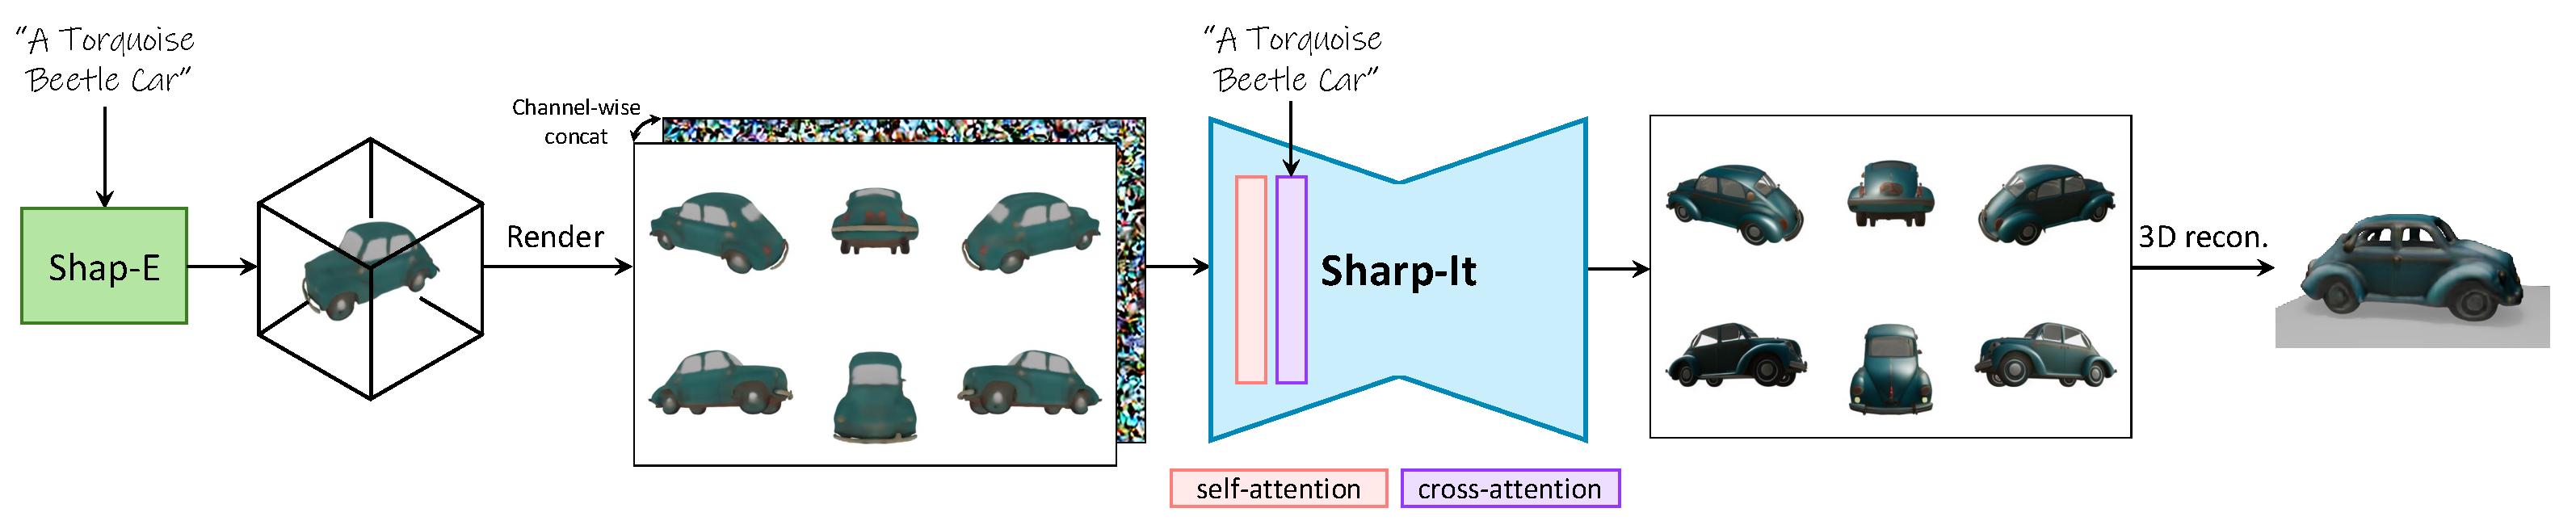
\includegraphics[width=\linewidth]{images/method_sharpe_new.pdf}
    \vspace{-18pt}
    \caption{Overview of 3D generation pipeline with Sharp-It.
    First, a 3D object is generated with Shap-E. Then, we render six views of this low-quality object. Sharp-It is a diffusion model based on Stable Diffusion~\cite{rombach2022highresolutionimagesynthesislatent} that enhances these views with the guidance of a text prompt by refining geometry and adding detailed appearance. Sharp-It employs cross-attention layers for text-based guidance and self-attention layers for cross-view consistency. A high-quality 3D object can be reconstructed from the multi-view image set.}
    \vspace{-12pt}
    \label{fig:method}
\end{figure*}
In this section, we present our approach to addressing the quality gap between direct 3D generative models and those that reconstruct 3D objects from multi-view images.
We focus on Shap-E~\cite{jun2023shape}, a 3D generative model, and introduce \emph{\ourname}, a multi-view-to-multi-view diffusion model that enhances 3D objects generated by Shap-E. We train \ourname{} to improve these objects by adding intricate appearance details and correcting geometric artifacts such as discontinuities and broken parts.
% We begin by providing the necessary background on Shap-E and Zero123++, the diffusion models upon which \ourname{} builds.
The process of generating a 3D model with \ourname{} is demonstrated in Figure~\ref{fig:method}.

\vspace{-2pt}
\subsection{Preliminaries}
\vspace{-2pt}

\paragraph{Shap-E} 
is a latent diffusion model specifically designed for generating 3D assets. As common in latent diffusion models~\cite{rombach2022highresolutionimagesynthesislatent}, Shap-E is trained in two stages. In the first stage, an encoder is trained to map 3D objects into a latent space. This latent space corresponds to the weight space of implicit functions that represent 3D shapes, with each shape represented as an element in $\mathbb{R}^{1024\times1024}$. The latent representation can be decoded using Signed Texture Field (STF) rendering, where it is treated as the weights of an implicit function.
In the second stage, a diffusion model is trained within the Shap-E latent space, allowing for conditioning on either text or images.

\vspace{-14pt}
\paragraph{Zero123++}
is an image-conditioned diffusion model designed to generate 3D-consistent multi-view images from a single input view~\cite{shi2023zero123singleimageconsistent}
}. It builds upon Stable Diffusion~\cite{rombach2022highresolutionimagesynthesislatent}, which is a latent diffusion model comprising a VAE and a UNet. The VAE encodes images into a resolution that is eight times smaller and consists of four channels, while the UNet serves as the diffusion model, operating on the four-channel latent codes.
Zero123++ is a fine-tuned version of Stable Diffusion that accepts an image as input. Given an input image, it produces a $3\times2$ grid of $320\times320$ pixel images, with six constant azimuth and elevation angles. 
Originally, Zero123++~\cite{shi2023zero123singleimageconsistent} was designed to generate this grid image with a grey background. In InstantMesh~\cite{xu2024instantmesh}, it was further fine-tuned to render a white background, addressing the issue of ``floaties''—particles floating through space during 2D-to-3D lifting.

\vspace{-3pt}
\subsection{Dataset Construction} \label{sec:data}
\vspace{-3pt}
We begin by constructing a paired dataset consisting of degraded Shap-E objects along with corresponding high-quality objects. Our key idea in constructing the dataset is that such pairs can be obtained by employing the encoder of Shap-E in conjunction with a high-quality 3D objects dataset.
Specifically, we utilize objects from Objaverse~\cite{deitke2023objaversexluniverse10m3d}, provided by~\cite{luo2023scalable, luo2024view}, and encode them using Shap-E's encoder. For each pair of an object from Objaverse and its encoded Shap-E latent code, we render a $3\times2$ grid from six predefined camera views, applying three HDR lighting conditions. Our experiments, detailed in the ablation studies, indicate that rendering each object under varying HDR lighting enhances the model’s performance.

We apply a filtering criteria on the resulting dataset.
We remove objects where the degraded Shap-E rendering is significantly different from the original object's rendering, indicating a failure of Shap-E's encoder. Additionally, we filter out objects that are too thin or do not match certain keywords based on their annotated captions. For each remaining object, we extract a caption using BLIP2~\cite{li2023blip2}.
Finally, we split the dataset into training and test sets, resulting in 180,000 objects for training and 6,000 for testing.


\vspace{-3pt}
\subsection{\ourname}
\vspace{-3pt}
\ourname{} is a multi-view to multi-view diffusion model designed to enhance low-quality multi-view images of 3D objects generated by Shap-E. It takes as input a set of multi-view images rendered from a low-quality 3D object, along with a textual prompt, and produces high-quality multi-view images with refined geometric details and textures that correspond to the input views.
% In practice, the multi-view image set is organized as a grid of $3\times2$ views, resulting in a total resolution of $960\times640$. Each view has its own azimuth and elevation angles, which remain fixed across different objects. 
An overview of a 3D generation pipeline with \ourname{} is shown in Figure~\ref{fig:method}.

\paragraph{Architecture}
The architecture of \ourname{} has two key requirements: generating multi-view image sets and incorporating input multi-view sets as conditions. We build on Zero123++~\cite{shi2023zero123singleimageconsistent, xu2024instantmesh}, which was fine-tuned for multi-view generation, where images are arranged in a $3\times2$ grid with a total resolution of $960\times640$ and fixed camera angles across objects.
%
To enable multi-view conditioning, we modify the architecture of Zero123++ by expanding the UNet input to 8 channels: 4 for latent noise and 4 for the VAE-encoded Shap-E multi-view images. This design lets our model leverage the coarse geometry from the input views to achieve better 3D consistency, and is inspired by image editing techniques that fine-tune diffusion models to accept an image as input and modify specific parts while preserving others~\cite{brooks2022instructpix2pix, rombach2022highresolutionimagesynthesislatent, yang2022paint}. Unlike these approaches, which operate on a single image, our model learns to enhance the input views in a 3D consistent manner. 
Furthermore, we replace Zero123++'s image embedding with text prompts in the cross-attention layers, enabling better enhancement control and appearance editing capabilities (Section~\ref{sec:app-edit}).


The model we build on consists of self-attention layers, which play an important role in facilitating the consistency of our produced multi-view set~\cite{shi2024mvdream, wang2023imagedream}. Since our model operates on a multi-view image grid, these layers can be seen as an application of cross-view attention between the different views. Similarly to previous works~\cite{wang2023imagedream, shi2024mvdream, shi2023zero123singleimageconsistent}, this allows our model to simultaneously refine corresponding points across different views by learning the correspondences between them. 
We visualize the learned correspondences in Figure~\ref{fig:cross-view-attention}. The figure displays self-attention maps for a query point marked by a red dot in the leftmost image. The results demonstrate that this point on the wheel receives the highest attention weight across different views. Additionally, the attention mechanism identifies semantically similar points -- notably, other wheels of the car.

\vspace{-14pt}
\paragraph{Training}

\begin{figure}
    \centering
    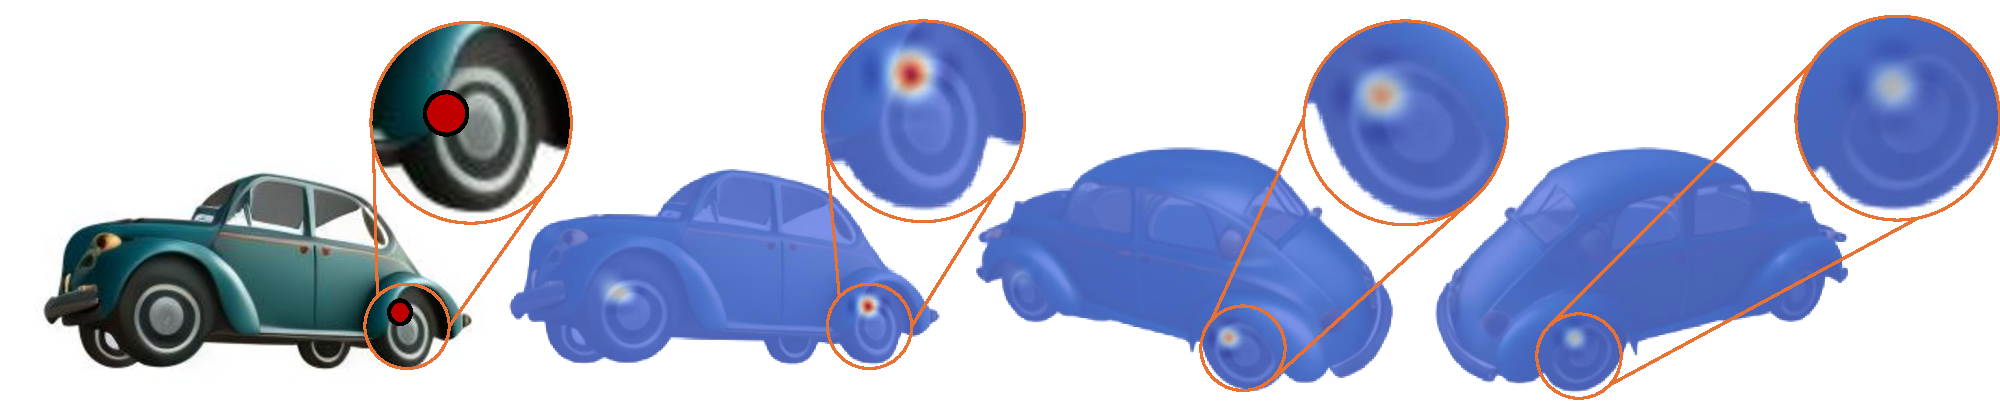
\includegraphics[width=0.99\linewidth]{images/cross-view-attention.pdf}
    \vspace{-10pt}
    \caption{Self-attention maps for a query point (red) on the car's wheel, showing highest attention weights at corresponding wheel locations across different views.}
    \vspace{-14pt}
    \label{fig:cross-view-attention}
\end{figure}

To train \ourname, we utilize our paired dataset consisting of $x$, a highly-detailed multi-view image set; $x_{\text{Shap-E}}$, a degraded version of $x$, representing the low-quality multi-view image generated by Shap-E; and a text prompt $c_{\text{prompt}}$, describing the high-quality 3D object.
We initialize \ourname{} with the weights of Zero123++ taken from the version trained by Xu \etal~\cite{instant3d2023}, and fine-tune it using standard diffusion training with v-prediction. The training loss is formulated as follows:
\[
\mathcal{L} = \mathbb{E}_{t, \epsilon \sim \mathcal{N}(0,1)} \left[ \| v - v_\theta(x_t, x_{\text{Shap-E}} \, ,c_{\text{prompt}}) \|^2 \right],
\]
where $v_\theta$ denotes the v-prediction of the model, parameterized by $\theta$. $x_t$ is obtained by adding noise to $x$ with respect to the diffusion timestep $t$. $t$ and $\epsilon$ are randomly sampled diffusion step and Gaussian noise, respectively. $v$ is defined as $\alpha_t\epsilon - \sigma x$, where $\alpha_t, \sigma$ are parameters of the noise scheduler.
We train our network for 500,000 steps, with a CFG drop probability of 0.1, and a batch size of 3 multi-views, using a single NVIDIA A6000 GPU. 
% The AdamW optimizer is employed, with a learning rate of $10^{-5}$.

\vspace{-10pt}
\paragraph{Inference}
Given a 3D object produced by Shap-E, we first render it from our six predefined azimuths and elevations to form \( x_{\text{Shap-E}} \). To enhance this multi-view image set, we sample a noisy image $x_T \sim \mathcal{N}(0, 1)$ and concatenate it channel-wise to \( x_{\text{Shap-E}} \) to create an 8-channel input to the model. 
The prompt used at inference time can be either the prompt used to generate the object with Shap-E or any other prompt that fits to the object, where the latter option is used to edit the appearance of the object.
We use our trained \ourname{} to iteratively denoise $x_t$, moving from the complete noisy multi-view image set, $x_T$ at $t=T$ to a clean, high-quality multi-view set $\hat{x}$ at $t=0$. The final output multi-view set $\hat{x}$ balances the information from the prompt $c_{\text{prompt}}$ and the degraded multi-view input $x_{\text{Shap-E}}$.

Our enhanced multi-view set can be reconstructed into a 3D object using any existing feed-forward sparse reconstruction method~\cite{xu2024instantmesh, jin2024lvsmlargeviewsynthesis, zhuang2024gtr, zhang2024geolrm}. 
In our experiments, we use InstantMesh~\cite{xu2024instantmesh} for reconstruction and provide its results in the supplementary materials.